% !TeX program = xelatex
\documentclass[UTF8,a4paper,11pt,fontset=fandol]{ctexart}
\usepackage[margin=1.8cm,top=2cm,bottom=2cm]{geometry}
\usepackage{amsmath,amssymb,booktabs,array,tabularx,xcolor,listings}
\usepackage{caption,graphicx,float}
\usepackage[unicode,colorlinks=true,linkcolor=blue!55!black,urlcolor=blue!55!black]{hyperref}
\usepackage{xurl}
\hypersetup{pdftitle={Lab 3 实验报告：划分与宏单元布局规划},pdfauthor={Tongbin Zhao}}
\setlength{\parindent}{2em}
\setlength{\parskip}{0.25em}
\setlength{\tabcolsep}{5pt}
\renewcommand{\arraystretch}{1.2}
\setlength{\emergencystretch}{2em}
\linespread{1.08}
\ctexset{section={format=\Large\bfseries,beforeskip=1.2ex,afterskip=.8ex},
  subsection={beforeskip=1ex,afterskip=.5ex}}
\newcommand{\code}[1]{\texttt{\detokenize{#1}}}
\captionsetup{font=small,labelfont=bf}
\lstdefinestyle{script}{language=Python,basicstyle=\ttfamily\small,
  keywordstyle=\color{blue!60!black},commentstyle=\color{green!35!black},
  numbers=left,numberstyle=\tiny\color{gray},numbersep=6pt,breaklines=true,
  columns=fullflexible,keepspaces=true,showstringspaces=false,
  frame=single,rulecolor=\color{gray!40},xleftmargin=1.7em}
\title{Lab 3 实验报告\\\large 划分与宏单元布局规划}
\author{Tongbin Zhao\\学号：2300012831}
\date{2026 年 11 月 10 日}
\begin{document}
\pagestyle{plain}
\begin{center}
{\LARGE\bfseries Lab 3 实验报告}\\[.4em]
{\large 划分与宏单元布局规划}\\[.6em]
Tongbin Zhao\quad 学号：2300012831\quad 2026 年 11 月 10 日
\end{center}
本报告完成 KL、FM、最大流增广和序列对布局的计算，并实现基于 ODB 输入的宏单元布局程序。
问题 1 使用精确有理数避免并列增益的浮点歧义；问题 2 通过约束图最长路径给出最小面积布局；
问题 3 记录实际 OpenROAD 运行结果。全部计算和运行入口位于提交目录的 \code{src/} 中。

\section{问题 1：划分}
\subsection{(a) 一轮 KL}
每条大小为 $k$ 的超边展开成边权 $1/(k-1)$ 的 clique，平行边相加。
其中 $de$ 同时出现于 $n_2$ 与 $n_5$，因此 $c_{de}=1/3+1/2=5/6$。
非零边权完整列为：
\begin{center}
\begin{tabular}{cl}
\toprule
边权 & 无向边 \\\midrule
$1/3$ & $bd,be,bf,df,ef$ \\
$1/2$ & $ab,ac,bc,cf,cg,dh,eh,fg$ \\
$5/6$ & $de$ \\
$1$ & $ag,fh$ \\\bottomrule
\end{tabular}
\end{center}
初始割为 $C_0=13/3$，初始 $D$ 值按 $a,b,c,d,e,f,g,h$ 排列为
\[
\left(0,-\frac23,0,\frac43,\frac13,-\frac23,1,-1\right).
\]
交换增益为 $g(u,v)=D_u+D_v-2c_{uv}$。每步交换后锁定两个顶点，
从新划分重新计算未锁顶点的 $D$，得到表~\ref{tab:kl}。
\begin{table}[H]\centering
\caption{KL 的完整四次交换。割值为加权图割。}\label{tab:kl}
\begin{tabular}{cccccl}
\toprule
步骤 & 交换对 & 本步增益 & 累计增益 & 割值 & 交换后的块 0 \\\midrule
0 & -- & -- & $0$ & $13/3$ & $\{a,b,c,d\}$ \\
1 & $(d,g)$ & $7/3$ & $7/3$ & $2$ & $\{a,b,c,g\}$ \\
2 & $(b,f)$ & $-1$ & $4/3$ & $3$ & $\{a,c,f,g\}$ \\
3 & $(a,h)$ & $-1$ & $1/3$ & $4$ & $\{c,f,g,h\}$ \\
4 & $(c,e)$ & $-1/3$ & $0$ & $13/3$ & $\{e,f,g,h\}$ \\\bottomrule
\end{tabular}
\end{table}
第 2 步前，$(D_a,D_b,D_c,D_e,D_f,D_h)=(-2,0,-1,-4/3,-1/3,-2)$，
因此 $g(b,f)=0-1/3-2/3=-1$。第 3 步前，
$(D_a,D_c,D_e,D_h)=(-1,-1,-4/3,0)$，$(a,h)$ 与 $(c,h)$ 同为 $-1$，
按字典序选择 $(a,h)$。第 4 步只剩 $(c,e)$。

最大累计增益 $7/3$ 首次出现在前缀长度 1，故回滚后三次交换，保留 $(d,g)$：
\[
\boxed{P_{\rm KL}=\{a,b,c,g\mid d,e,f,h\},\qquad C_{\rm KL}=2.}
\]

\clearpage
\subsection{(b) 一轮 FM}
现在直接使用原始无权超图，每条跨块超边只计 1。
初始跨块超边为 $n_2,n_3,n_4,n_5$，所以 $C_0=4$。
初始单点增益按 $a,b,c,d,e,f,g,h$ 排列为 $(0,-1,0,1,0,-1,1,-1)$；
$d,g$ 并列，先移动 $d$。移动后块大小为 $3:5$，下一步只能从块 1 移入块 0。

\begin{table}[H]\centering
\caption{FM 的完整移动过程。箭头表示从原块移往另一块。}
\begin{tabular}{cccccl}
\toprule
步骤 & 单元及方向 & 增益 & 割值 & 大小 $(|B_0|,|B_1|)$ & 移动后的块 0 \\\midrule
0 & -- & -- & 4 & $(4,4)$ & $\{a,b,c,d\}$ \\
1 & $d:0\to1$ & 1 & 3 & $(3,5)$ & $\{a,b,c\}$ \\
2 & $g:1\to0$ & 1 & 2 & $(4,4)$ & $\{a,b,c,g\}$ \\
3 & $b:0\to1$ & 0 & 2 & $(3,5)$ & $\{a,c,g\}$ \\
4 & $f:1\to0$ & $-1$ & 3 & $(4,4)$ & $\{a,c,f,g\}$ \\
5 & $h:1\to0$ & 0 & 3 & $(5,3)$ & $\{a,c,f,g,h\}$ \\
6 & $a:0\to1$ & $-1$ & 4 & $(4,4)$ & $\{c,f,g,h\}$ \\
7 & $c:0\to1$ & 0 & 4 & $(3,5)$ & $\{f,g,h\}$ \\
8 & $e:1\to0$ & 0 & 4 & $(4,4)$ & $\{e,f,g,h\}$ \\\bottomrule
\end{tabular}
\end{table}
第 3 步 $b$ 与 $f$ 增益同为 0，选 $b$；第 6 步块大小为 $5:3$，
虽然 $e$ 的增益为 0，但移动 $e$ 将产生 $6:2$，因此非法。
合法的 $a,c$ 增益同为 $-1$，选 $a$。第 7 步 $c,e$ 同为 0，选 $c$。
第 8 步后所有单元均锁定，停止。

最小割 2 首次出现在前缀长度 2（长度 3 也达到 2，但不是首次），故只保留 $d,g$：
\[
\boxed{P_{\rm FM}=\{a,b,c,g\mid d,e,f,h\},\qquad C_{\rm FM}=2.}
\]
此时只有 $n_2=\{b,d,e,f\}$ 与 $n_3=\{c,f,g\}$ 跨块。
KL 和 FM 恰好得到相同划分；前者优化加权图割，后者优化超边割数，两种目标并不等同。

\subsection{(c) 一次 BFS 增广}
将每条无向边替换成两个等容量有向弧，所有原始弧初始流量均为 0。
从 $a$ 开始按邻点字母顺序扫描：$a$ 发现 $b,c,g$，$b$ 发现 $d,e,f$，
随后依次展开 $c,g,d$，在扫描 $d$ 时首次发现 $h$ 并停止。
发现顺序为 $(a,b,c,g,d,e,f,h)$，父指针给出
\[
\boxed{a\to b\to d\to h,\qquad
\Delta=\min\{1/2,1/3,1/2\}=1/3.}
\]
\begin{center}
\begin{tabular}{ccccc}
\toprule
路径弧 & 容量 & 更新后流量 & 正向剩余容量 & 反向合并剩余容量 \\\midrule
$a\to b$ & $1/2$ & $1/3$ & $1/6$ & $5/6$ \\
$b\to d$ & $1/3$ & $1/3$ & $0$ & $2/3$ \\
$d\to h$ & $1/2$ & $1/3$ & $1/6$ & $5/6$ \\\bottomrule
\end{tabular}
\end{center}
反向原始弧的流量仍为 0；表中最后一列将它的剩余容量 $c_{uv}$
与可撤销本次正向流量的反向残量 $\Delta$ 合并，即 $c_{uv}+\Delta$。
若使用独立残量弧表示，二者分别为 $c_{uv}$ 与 $1/3$。

\clearpage
\section{问题 2：序列对}
\subsection{(a) 水平约束图}
采用题目给定的序列对与方向定义。设模块 $i$ 的 0 起始序号为 $(p_i,n_i)$，
图中网格坐标为 $(p_i+n_i-7,n_i-p_i)$，因此 1 在顶点、8 在底点。
网格用于表达序列次序，并非模块实际布局坐标。
\begin{figure}[H]\centering
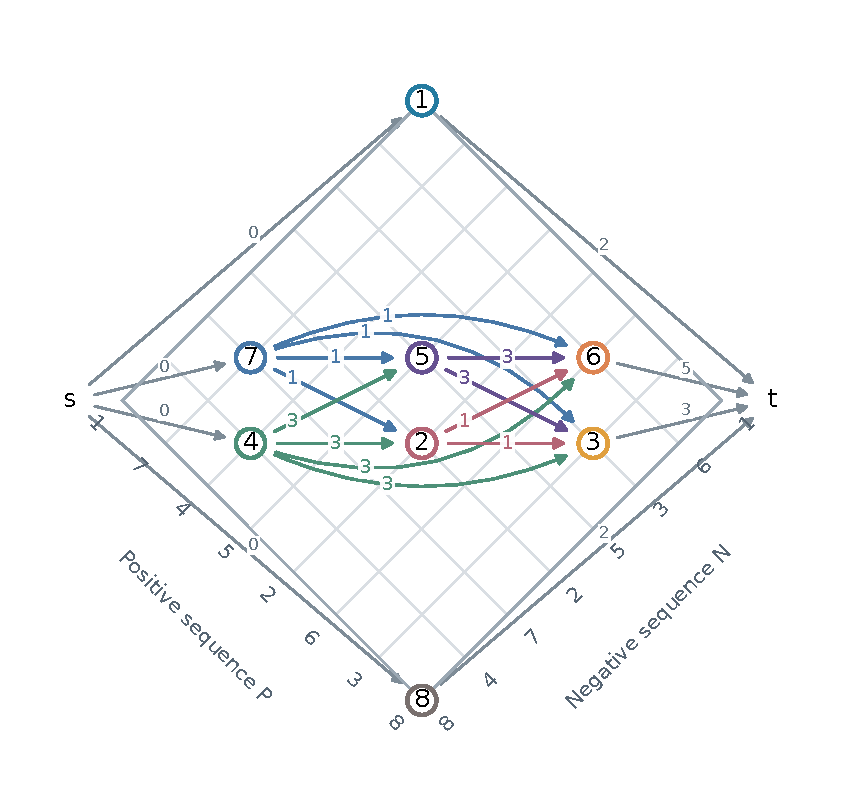
\includegraphics[width=.93\linewidth]{asset/horizontal_graph.pdf}
\caption{完整水平约束图。彩色弧为模块间约束，边权为起点宽度；灰色弧连接虚拟源点与汇点。}
\end{figure}
为便于核对图中交叉的边，将全部 12 条模块间水平边列为邻接表。
同一行每条出边都具有表中权重。
\begin{center}
\begin{tabular}{ccc|ccc}
\toprule
起点 & 终点集合 & 权重 & 起点 & 终点集合 & 权重 \\\midrule
7 & $\{2,3,5,6\}$ & 1 & 4 & $\{2,3,5,6\}$ & 3 \\
5 & $\{3,6\}$ & 3 & 2 & $\{3,6\}$ & 1 \\\bottomrule
\end{tabular}
\end{center}
源点 $s\to\{1,4,7,8\}$ 的边权为 0；
$1,3,6,8\to t$ 的权重依次为 $2,3,5,2$。

\clearpage
\subsection*{(a) 垂直约束图}
\begin{figure}[H]\centering
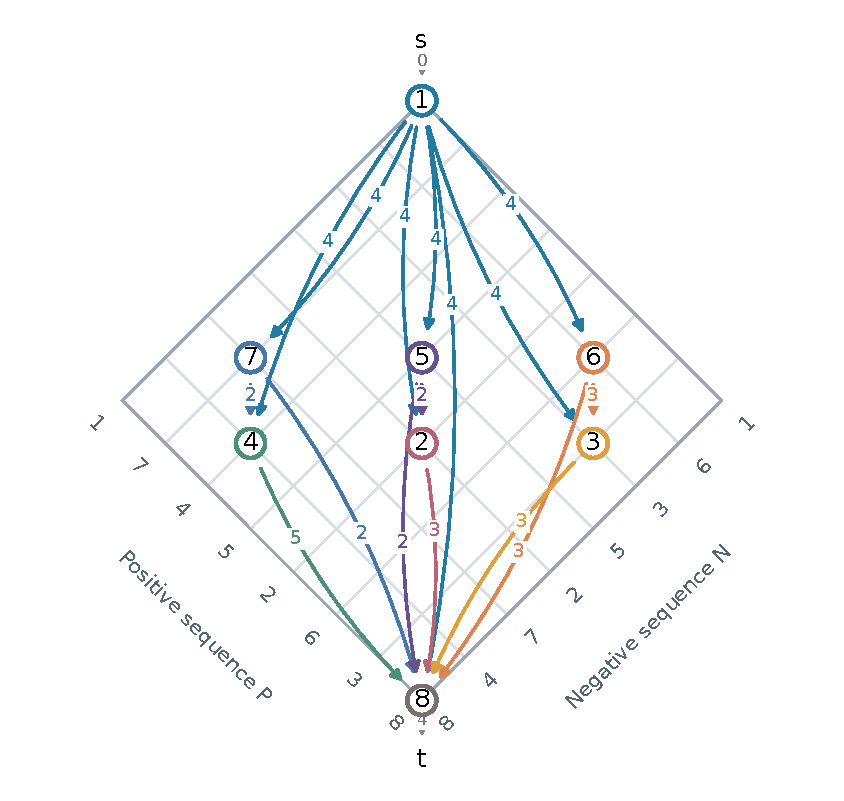
\includegraphics[width=.93\linewidth]{asset/vertical_graph.pdf}
\caption{完整垂直约束图。$i\to j$ 表示 $i$ 在 $j$ 下方，权重为 $h_i$；图上向下的箭头仅表示序列网格中的有向关系。}
\end{figure}
全部 16 条模块间垂直边如下。虚拟源点边为 $s\to1$（权重 0），
汇点边为 $8\to t$（权重 4）。
\begin{center}
\begin{tabular}{ccc}
\toprule
起点 & 终点集合 & 权重 \\\midrule
1 & $\{2,3,4,5,6,7,8\}$ & 4 \\
7 & $\{4,8\}$ & 2 \\
4 & $\{8\}$ & 5 \\
5 & $\{2,8\}$ & 2 \\
2 & $\{8\}$ & 3 \\
6 & $\{3,8\}$ & 3 \\
3 & $\{8\}$ & 3 \\\bottomrule
\end{tabular}
\end{center}
两个图的全部边都沿正序列 $P$ 前进，故 $P$ 同时是两个图的拓扑序。
任意两个模块恰好由一条水平边或垂直边确定关系，共 $12+16=\binom82=28$ 对。

\clearpage
\subsection{(b) 相对位置表}
表头与题目 Figure 2 一致：第 $i$ 行的 Left-of 集合为
“$i$ 在这些模块的左侧”，Below 集合为“$i$ 在这些模块的下方”；
Right-of、Above 同理。这样第 1 行的 Below 包含其余 7 个模块，与题目给出的示例一致。
\begin{table}[H]\centering
\caption{序列对规定的相对位置，不依赖最终布局中的额外几何关系。}
\begin{tabular}{ccccc}
\toprule
模块 & Left-of & Right-of & Above & Below \\\midrule
1 & $\varnothing$ & $\varnothing$ & $\varnothing$ & $\{2,3,4,5,6,7,8\}$ \\
2 & $\{3,6\}$ & $\{4,7\}$ & $\{1,5\}$ & $\{8\}$ \\
3 & $\varnothing$ & $\{2,4,5,7\}$ & $\{1,6\}$ & $\{8\}$ \\
4 & $\{2,3,5,6\}$ & $\varnothing$ & $\{1,7\}$ & $\{8\}$ \\
5 & $\{3,6\}$ & $\{4,7\}$ & $\{1\}$ & $\{2,8\}$ \\
6 & $\varnothing$ & $\{2,4,5,7\}$ & $\{1\}$ & $\{3,8\}$ \\
7 & $\{2,3,5,6\}$ & $\varnothing$ & $\{1\}$ & $\{4,8\}$ \\
8 & $\varnothing$ & $\varnothing$ & $\{1,2,3,4,5,6,7\}$ & $\varnothing$ \\\bottomrule
\end{tabular}
\end{table}
\subsection{(c) 最小面积布局}
沿 $P$ 顺序计算两个约束图的最长路径，得到下表所列左下角坐标。模块均不旋转，边界可接触。
\begin{minipage}{.44\linewidth}\centering
\begin{tabular}{ccc}
\toprule
模块 & $(w_i,h_i)$ & $(x_i,y_i)$ \\\midrule
1 & $(2,4)$ & $(0,0)$ \\
2 & $(1,3)$ & $(3,6)$ \\
3 & $(3,3)$ & $(6,7)$ \\
4 & $(3,5)$ & $(0,6)$ \\
5 & $(3,2)$ & $(3,4)$ \\
6 & $(5,3)$ & $(6,4)$ \\
7 & $(1,2)$ & $(0,4)$ \\
8 & $(2,4)$ & $(0,11)$ \\\bottomrule
\end{tabular}
\end{minipage}\hfill
\begin{minipage}{.52\linewidth}\centering
\captionsetup{hypcap=false}
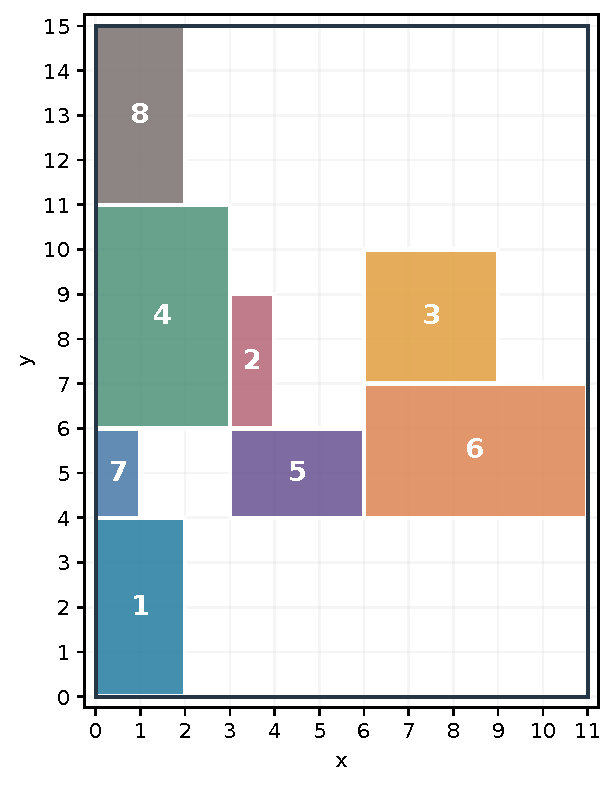
\includegraphics[height=7.8cm]{asset/problem2_packing.pdf}
\captionof{figure}{满足给定序列对的紧凑布局。}
\end{minipage}

水平路径 $4\to5\to6\to t$ 强制 $W\ge3+3+5=11$；
垂直路径 $1\to7\to4\to8\to t$ 强制 $H\ge4+2+5+4=15$。
图中布局同时达到这两个下界，因此对于给定序列对，
\[
\boxed{W=11,\quad H=15,\quad WH=165}
\]
是全局最小面积；所有坐标为非负整数。
·
\clearpage
\section{问题 3：OpenROAD 宏单元布局}
\subsection{实现与复杂度}
\code{hw3.py} 在 OpenROAD Python 中读取真实的 \code{2_1_floorplan.odb}，
动态获取所有 \code{BLOCK} 实例、主单元尺寸、引脚中心和至少含两个宏引脚的网络。
不硬编码六个实例名，不读取冻结 fixture；fixture 只由原版 \code{check.py} 用于独立检查。

\paragraph{序列对打包。}
先构造 $N$ 的位置表，对 $P$ 中的每一对 $i,j$（$i$ 在前）判断：
若 $n_i<n_j$，加入水平边 $i\to j$，边权 $w_i+35$；否则加入垂直边，边权 $h_i+35$。
全部边沿 $P$ 前进，因此无需额外拓扑排序。坐标初值为 0，按 $P$ 松弛：
\[
x_j\leftarrow\max(x_j,x_i+w_i+35),\qquad
y_j\leftarrow\max(y_j,y_i+h_i+35).
\]
每条路径都给出一个坐标下界，最长路径达到全部约束下的逐坐标最小值。
每对模块有一个轴上的间距约束，因此不会重叠且至少保持 $35\,\mu$m 间距。
构图及最长路径各为 $O(n^2)$ 时间，显式邻接表占 $O(n^2)$ 空间。
报告的打包尺寸按照模板接口包含右侧和顶部 halo：
\[
W=\max_i(x_i+w_i+35),\qquad H=\max_i(y_i+h_i+35).
\]
输出时整体平移到 $(x_{\rm core}+5,y_{\rm core}+5)$；四种合法朝向不交换宽高。

\paragraph{引脚变换与 HPWL。}
设 R0 下引脚偏移为 $(p_x,p_y)$，主单元宽高为 $(w,h)$，则
\begin{center}
\begin{tabular}{ccccc}
\toprule
朝向 & R0 & MX & MY & R180 \\\midrule
偏移 & $(p_x,p_y)$ & $(p_x,h-p_y)$ & $(w-p_x,p_y)$ & $(w-p_x,h-p_y)$ \\\bottomrule
\end{tabular}
\end{center}
加上宏的实际左下角后，每条网络贡献
$(\max X-\min X)+(\max Y-\min Y)$。遍历全部网络的宏引脚，
时间复杂度为 $O(\sum_e |e|)$；同一宏的不同引脚仍分别计入。

\paragraph{模拟退火与目标函数。}
沿用模板的三类扰动：以 $0.35/0.35/0.30$ 的概率交换 $P$/交换 $N$/改变一个朝向，
温度从 5000 指数下降至 20。主要代价为
\[
C=\operatorname{HPWL}_{\rm macro}
 +10^5\bigl([W-W_{\rm avail}]_+ +[H-H_{\rm avail}]_+\bigr),
\]
其中可用宽高为核心区宽高减去两侧各 $5\,\mu$m。
保存最优解时按 $(C,WH)$ 的字典序比较：面积只在主代价相同时破同分。
模板的 $10^{-3}WH$ 加权项已移除，防止用更大 HPWL 换取较小面积。
最终输出前再次检查打包外框约束，失败时抛出异常而非输出越界布局。

\paragraph{验证与复现。}
7 项标准库单元测试覆盖：给定八模块的已知最优解、100 组随机序列对的独立反复松弛验证、
非法排列、四朝向与平移不变性、同宏多引脚、面积代价规则，以及问题 1 的精确结果。
提交 runner 修正了相对 ORFS 路径在切换工作目录后的解析，以及超时日志的字节串解码；
布局命令、checker 和验收门限保持题目原值。

\clearpage

\subsection{实测环境与布局结果}
本次使用 Docker 的 Linux/amd64 环境；OpenROAD 版本为
\code{26Q3-1985-gc3e680b01b}，Python 版本为 3.10.12。
ORFS 源码版本为 \code{5b87982c6133}。
容器固定到 \code{openroad/orfs:26Q3-565-gef7fbfb0e} 对应的镜像摘要，
完整摘要及命令见提交 README 和 \code{environment.json}。
实际读取到 6 个宏、127 条宏网络，核心区域为
$(2.300,2.720)$ 至 $(2680.880,3484.320)\,\mu$m。
退火参数为 seed=0、100,000 次迭代，搜索耗时 20.3 s。

\begin{table}[H]\centering
\caption{实际运行指标。全设计 HPWL 来自 detailed\_placement 的 legalized HPWL。}
\begin{tabular}{lr}
\toprule 指标 & 实测值 \\\midrule
宏网络 HPWL & 102,840.185 $\mu$m \\
打包宽度 $W$ / 高度 $H$（含外侧 halo） & 2,249.690 / 2,994.360 $\mu$m \\
详细布局后全设计 HPWL & 647,866.4 $\mu$m \\
题目提供的 RTLMP 基准 & 738,243.9 $\mu$m \\
与题目基准之比 / 降低比例 & 0.877578 / 12.242\% \\
验收门限 / checker 结果 & 730,000 $\mu$m / \textbf{PASS} \\\bottomrule
\end{tabular}
\end{table}
下游严格执行题目给定的 \code{place_pins}、密度 0.6 的 \code{global_placement}
及 \code{detailed_placement}。宏几何检查和最终检查均输出 \code{RESULT: PASS}。
这里的比值以题目固定的 738,243.9 $\mu$m 为分母；其标注的 OpenROAD 版本为
\code{26Q3-1510-g6cb3f2b704}，与本次工具版本存在差异，因此不将这一比值解释为严格同版本的算法对比。

\begin{figure}[H]\centering
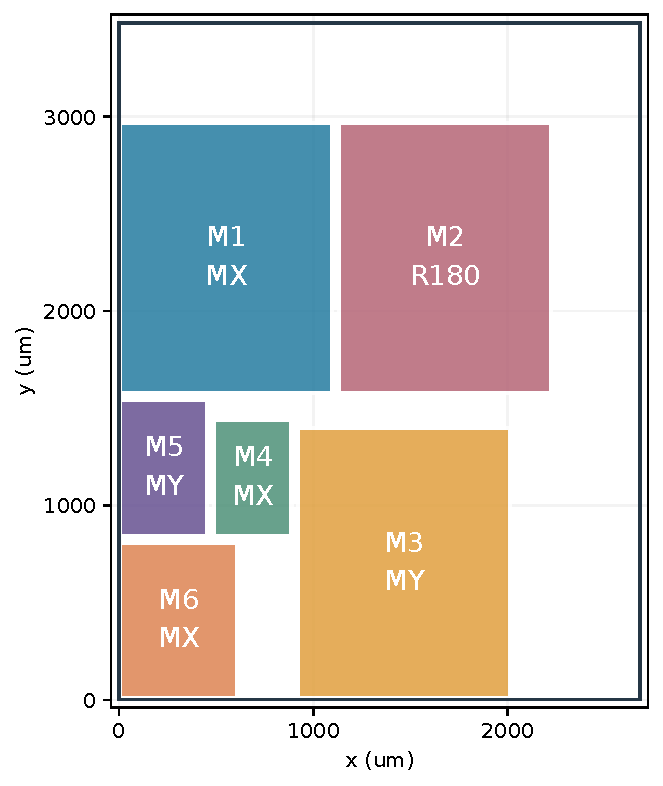
\includegraphics[height=9.2cm]{asset/macro_floorplan.pdf}
\caption{输出的宏布局。外框为核心区，矩形为实际宏边界；编号和坐标见下页。}
\end{figure}
最优序列为 $P=(M_{6},M_{5},M_{4},M_{3},M_{1},M_{2})$，$N=(M_{1},M_{2},M_{5},M_{4},M_{6},M_{3})$。

\clearpage
\subsection{宏坐标与面积平衡划分}
\begin{table}[H]\centering\small
\caption{写入 JSON/Tcl 的位置与朝向，单位为 $\mu$m。实际 ODB 名称中的方括号转义由程序保留。}
\begin{tabular}{clrrc}
\toprule 编号 & 实例（此处省略反斜杠转义） & $x$ & $y$ & 朝向 \\\midrule
$M_{1}$ & \code{RAM.genblk1[0].RAM} & 7.300 & 1577.720 & MX \\
$M_{2}$ & \code{RAM.genblk1[1].RAM} & 1132.145 & 1577.720 & R180 \\
$M_{3}$ & \code{RAM.genblk1[2].RAM} & 923.000 & 7.720 & MY \\
$M_{4}$ & \code{ahb_sys_0_uut.S0.CACHE} & 490.390 & 842.720 & MX \\
$M_{5}$ & \code{ahb_sys_0_uut.apb_sys_inst_0} & 7.300 & 842.720 & MY \\
$M_{6}$ & \code{ibex_core} & 7.300 & 7.720 & MX \\
\bottomrule
\end{tabular}
\end{table}
每个 RAM 的面积为 $1,514,187.0492\,\mu\mathrm{m}^2$；
Cache、APB、Ibex 的面积依次为 $238,566$、$313,663$、$480,000\,\mu\mathrm{m}^2$。
总面积 $A=5,574,790.1476\,\mu\mathrm{m}^2$。
“在一半面积的 $\pm10\%$ 内”对应每块面积落在 $[0.45A,0.55A]$，即
\[
[2\,508\,655.5664,\ 3\,066\,134.5812]\,\mu\mathrm{m}^2.
\]
固定一个宏在块 A 中可消除互补重复；穷举 $2^{6-1}-1=31$ 个非空无序划分，
恰有下表 3 种满足平衡约束。每条跨块宏网络只计一次。
\begin{table}[H]\centering\small
\caption{全部合法无序二分；交换块 A/B 不形成新划分。}
\begin{tabular}{ccrrc}
\toprule 块 A & 块 B & A 面积 & B 面积 & cut \\\midrule
$\{M_{1},M_{2}\}$ & $\{M_{3},M_{4},M_{5},M_{6}\}$ & 3,028,374.098 & 2,546,416.049 & 47 \\
$\{M_{1},M_{3}\}$ & $\{M_{2},M_{4},M_{5},M_{6}\}$ & 3,028,374.098 & 2,546,416.049 & 47 \\
$\{M_{1},M_{4},M_{5},M_{6}\}$ & $\{M_{2},M_{3}\}$ & 2,546,416.049 & 3,028,374.098 & 47 \\
\bottomrule
\end{tabular}
\end{table}
证明其完备性：无 RAM 的三个小宏总面积只有 $1,032,229$，不足下界；
三个 RAM 同块则超过上界。两个 RAM 的面积为 $3,028,374.0984$，
即使再加最小的 Cache 也会超过上界。因此一块必须恰含两个 RAM，另一块包含剩余 RAM 和全部小宏，
只有选择哪一个 RAM 单独与小宏同块这 3 种可能。两块相对半总面积的偏差均约为 $8.65\%$。

对真实 ODB 中的网络按其涉及的宏集合分组，得到：
\begin{center}
\begin{tabular}{lc}
\toprule 宏集合 & 网络数 \\\midrule
$\{M_{1},M_{2},M_{3}\}$ & 46 \\
$\{M_{1},M_{2},M_{3},M_{4},M_{5},M_{6}\}$ & 1 \\
$\{M_{4},M_{5},M_{6}\}$ & 25 \\
$\{M_{5},M_{6}\}$ & 55 \\
\bottomrule
\end{tabular}
\end{center}
三种平衡划分都分开三个 RAM，因此 46 条 RAM 共用网络全部跨块；
连接全部宏的 1 条网络也跨块；其余 $25+55=80$ 条网络只涉及三个小宏，它们始终同块。
故每个平衡划分的 cut 都等于 $46+1=47$，此平衡约束下无法进一步降低。

\clearpage
\subsection{代价函数的一个具体局限}
宏 HPWL 只统计至少含两个宏引脚的网络，会遗漏宏到标准单元或外部端点的连线；
对全部宏作相同平移，宏间 HPWL 不变，但这些被遗漏的线长可能明显变化。
下面用一个完全可计算的小例子说明：两个 $10\times10$ 宏只有一个中心引脚，
核心区为 $[0,200]\times[0,100]$，两宏左下角原为 $(5,5)$、$(50,5)$，间距恰为 $35$。
网络 $e_1$ 连接两个宏引脚，网络 $e_2$ 连接第一个宏引脚与固定端点 $(150,10)$。
将两个宏整体右移 80 后仍合法，得到：
\begin{center}
\begin{tabular}{lccc}
\toprule 布局 & $e_1$（宏代价） & $e_2$（被忽略） & 全部网络之和 \\\midrule
左下角 $(5,5),(50,5)$ & 45 & 140 & 185 \\
左下角 $(85,5),(130,5)$ & 45 & 60 & 105 \\\bottomrule
\end{tabular}
\end{center}
两者宏 HPWL 同为 45，宏集合的外包宽高也相同，但总 HPWL 相差 80。
当前最长路径打包固定在左下角，输出仅加固定 $5\,\mu$m 边界偏移，
因此既没有代价信息，也没有整体平移扰动来选择后者。
这里的固定端点是用于证明局限的简化外部引脚，并非将该数值当作 chameleon 的实测性能。

一种改进是从 ODB 纳入宏到标准单元/端口的网络，结合外部引脚的当前位置估计线长，
并加入合法的整体平移或局部松弛；不过标准单元还会在后续布局中移动，
因此最终仍须以详细布局后的全设计 HPWL 为验收依据。
本次采用题目要求的宏 HPWL 目标，并用完整下游流程验证所得解。

\subsection{运行产物}
\code{hw3_run/} 保存 \code{macro_placement.json/.tcl}、
\code{flow_report.json}、\code{student.log}、\code{flow.log}、
两份 checker 日志、\code{partition_analysis.json}、\code{search_config.json} 以及环境记录。
\code{3_2_place_custom.odb} 可由同一命令重新生成。
所有表格由这些文件自动提取；原始数据副本保存在报告的 \code{asset/} 目录。


\clearpage
\appendix
\section{AI 使用记录}
本次使用 Codex 完成了问题1和问题2的内容排版、问题3的编程debug和报告生成，以及最后的
提交压缩包整理。具体使用的prompt如下：
\begin{enumerate}
  \item 读取我发给你的手写pdf，这是问题1和问题2的回答。帮我提取相关信息之后排版到latex报告report/lab3_report.tex中
  \item 帮我看一下给出的annealing driver如何调用，给我一个调用的示例并说明输入输出的含义
  \item 检查我的pack实现，指出其中的算法逻辑错误在哪里
  \item 我已经跑出一个结果了，帮我看看它是否符合要求，如果符合要求，帮我生成编程部分的
  报告，整合进实验报告中。顺手解决一下latex语法和排版的问题
  \item 按照 HW3_problem.pdf 中的提交压缩包结构要求，帮我把需要提交的内容整理到handin文件夹下，我来压缩提交
\end{enumerate}
